\chapter{Optimización}

\section{Introducción}
La optimización consta de 3 etapas, la primera fue modelar el motor con los
coeficientes de descarga constantes extraidos de trabajos anteriores para tener
una primer aproximación de la geometría de los puertos.
%
A partir de estos resultados se obtuvo una geometría preliminar con nuevos
díametros, longitudes y ángulos.
%
La segunda etapa consiste en volcar los datos obtenidos en un programa de CAD,
para realizar una estimación de la forma de los puertos.
%
En el modelo de CAD se representaron varios elementos del motor, consiguiendo un
modelo dinámico del que se pueden extraer los volúmenes a simular en diferentes,
puesto que se parametrizaron variables como ángulos de cigüeñal, reglaje y
diámetros.
%
Los volúmenes se extraen como archivos ``.brep'' para ser importados en el
software SALOME, del cual se obtiene un \emph{stl} hermético con el algoritmo
NETGEN 1D-2D el cual se exporta como un ASCII STL, que puede ser leido por
OpenFOAM.

Con este programa se realizaron las flujometrías en diferentes condiciones
operativas del motor, para cada una de las posiciones del rotor seleccionadas.
%
A partir de estos datos se armó un mapa de coeficientes de descarga que se
utilizó en ICESym para modelar de manera más precisa el flujo de gas a través
los puertos de admisión y escape en diferentes condiciones operativas del motor.
%
La tercer etapa consta de volver a correr la optimización, con la nueva
geometría y con el mapa de descarga de los puertos como dato.

\section{Herramientas}
%
En las diferentes etapas de optimización se utilizaron herraminetas (software)
existente y nuevo, admás de realizar pequeñas modificaciones a ICESym para
facilitar la comunicación del optimizador.

\begin{itemize}
  %
  \item Optimización y comunicación con ICESym
  %
  \begin{itemize}
    \item aspiracion.m y mkport\_data.m, creado por ``chiquito'' para generar
      las curvas de alzada de los puertos
    \item motor.py, comunicación con ICESym
      %
    \item pip\_bin.py, contiene el algorimto genético
      %
    \item utils.py, utilidades varias
      %
  \end{itemize}
  %
  \item Flujometrías y mapa de $C_D$
    %
  \begin{itemize}
    %
    \item pre.py, lee los resultados de una simulación en particualr y prepara
      un archivo de condiciones iniciales para la flujometría con OpenFOAM
      %
    \item post.py, lee los resultados de una flujometría y calcula el caudal
      másico obtenido
      %
    \item mapa\_cd.py, construye un mapa de $C_D$ a partir de los de presión,
      alzada y caudal másico obtenidos
      %
  \end{itemize}
  %
  \item{Varios}
    %
  \begin{itemize}
    %
    \item rutinas\_termodinamicas\_motrices, se recopilaron de rutinas de octave
      de la cátedra de Máquinas Motrices I de la UNCo, calculan propiedades
      varias de la mezcla quemada y sin quemar.
      %
    \item geom.scad, script de OpenSCAD que constuye una modelo 3D de la
      geometría obtenida, pudiendo admeás crear archivos ``.gif''.
      %
  \end{itemize}
  %p
\end{itemize}



\section{Optimizador y Algoritmo genético}
%
\subsection{Algoritmo Genético}
%
Se seleccionó un algoritmo genético para realizar la optimización de la
geometría del MRCVC por la simplicidad y facilidad de implementación del mismo.
%
Si bien este tipo de métodos no garantizan que se alcance un resultado óptimo,
en la práctica\cite{goldberg}\cite{shi} se ha observado que alcanzan soluciones
muy cercanas a las óptimas tras pocas iteraciones del método.

Una de las ventajas de este método es que no requiere información del gradiente
de la función que se está evaluando, lo cual es útil cuando no se puede asegurar
la existencia de la derivada de la función en todo el dominio ó cuando se tiene
una función con más de un máximo o mínimo local.
%
Además, el punto de partida de la optimización es una población generada al
azar, de modo que se tiene un muestreo aleatorio del dominio que se está
evaluando.
%
Esto hace que el método sea poco susceptible a caer en un óptimo local.

Se puede decir que un algoritmo genético es un método de búsqueda aleatoria
guiada.
%
¿Cómo difieren los AG de los métodos tradicionales de búsqueda?
%
\begin{enumerate}
    %
  \item Los AG trabajan sobre una representación de las variables estudiadas y
    no necesariamente sobre las variables de estudio.
    %
    \item Trabajan con un conjunto de datos, no con un solo punto.
    %
    \item Utilizan una función objetivo para evaluar cada punto de datos, sin
      necesidad de conocer la derivada de la función que se está evaluando.
    %
    \item Los AG usan reglas probabilísticas, no deterministas.
    %
\end{enumerate}

Otros métodos de optimización se mueven de un punto al siguiente en el espacio
solución, basándose en alguna regla de decisión, esto puede ser riesgo porque se
puede caer en un óptimo local.
%

\subsection{Componentes de un AG}
%
El funcionamiento básico de estos algoritmos se sintetiza en el
pseudocódigo~\ref{algo:genetico}, basicamente hay tres operadores que son
suficientes para realizar este tipo de optimización: SELECCIÓN CRUZA Y MUTACIÓN.

%% \begin{enumerate}
%%     \item Selección
%%     \item Cruza
%%     \item Mutación
%% \end{enumerate}

La reproducción consiste en crear individuos a partir del puntaje que devuelve
en la función objetivo, la función objetivo es una medida del valor que
queremos optimizar.
%
Este paso significa que aquellos individuos que tengan valores, por ejemplo más
altos, de función objetivo tendrán más posibilidades de ser ``copiados'', de esta
forma se imita a la selección natural.

La cruza consiste en combinar los ``vectores'' de dos individuos para obtener uno
nuevo.

La mutación consiste en modificar aleatoriamente uno o más parámetros de cada
nuevo individuo.

Estos 3 simples mecanismos le dan a los AG su ¿poder?

La mutación juega un rol secundario pero muy importante, es secundario porque se
pueden alcanzar soluciones satisfactorias sin incluir este mecanismo, sin
embargo se utiliza con probabilidades pequeñas para evitar la pérdida temprana
de información relevante.
%
Si la probabilidad de mutación es muy alta, el AG se convierte en una simple
búsqueda aleatoria.


\begin{algorithm}
 \caption{Algoritmo de optimización}\label{algo:genetico}
     \SetAlgoLined
     iter = 0;
     Inicializar población.\;
     \While{No se cumpla cierta condición}{
     SELECCIÓN de los individuos más aptos.\;
     CRUZA los candidatos seleccioados (creación de la anueva población)\;
     MUTACIÓN algunos individuos de la nueva población\;
     iter = iter + 1\;
     }
     {Guardar resultados\;}
\end{algorithm}


\subsection{\emph{Schema} y paralelismo implícito}

\emph{Schema} o esquema es una plantilla, un subconjunto de los parámetros que
definen al individuo en un AG que contienen información relevante al problema
en estudio.
%
Estas plantillas surgen de similitudes en posiciones y valores que dan buena
aptitud a un individuo.
%
Un AG procesa $n$ individuos y $n^k$ \emph{schematas} por
iteración~\cite{goldberg}, cuanto mayor sea el tamaño del \emph{schema}, mayor
la probabilidad de ser truncado durante la cruza o mutación, esto produce que
los
patrones de menor tamaño tengan mayor probabilidad de supervivencia de una
generación a otra.
%
Este proceso en el que bloques de información de menor tamaño al total de
parámetros que se está evaluado sobreviven de una generación a otra sin
necesidad de ingresar alguna modificación algoritmo es conocido como paralelismo
implícito.


\subsection{Implementación}
%
Gran parte de este trabajo fue utilizar a ICESym como parte de la función con la
que se evalúan los motores.
%
Para lograr esto se modificó parte del código de ICESym, con el objetivo de
facilitar la lectura de los resultados que arroja el simulador.
%
Además, se es necesario poder ejecutar de manera automatica una simulación con
una configuración particular del motor.
%
Otro aspecto del optimizador que se desarrolló es el de poder ejecutar múltiples
instancias de ICESym en paralelo para reducir el tiempo de ejecución cada
simulación.


Para la primer iteración se programaron los algoritmos y funciones necesarias
para llevar a cabo la optimización desde cero.
%
Posteriormente se tomo la la librería DEAP~\cite{DEAP_JMLR2012} y se
modificaron los operadores a medida, para poder utilizarlos con ICESym.

\subsubsection{Población}



































El optimizador se construyó a partir de la librería DEAP\cite{DEAP_JMLR2012}, la
cual contiene operadores y algoritmos disponibles para realizar una optimización
de este tipo.

Las funciones para que el optimizador pueda controlar y comunicarse con ICESym
se encuentran en el archivo ``motor.py'', una de las funcionalidades ``destacadas''
es la posibilidad de ejecutar múltiples instancias del simulador en paralelo, esto
fue clave para reducir el timpo de ejecución de las corridas de optimización.
%
La ejecución en paralelo de ICESym consiste en separar la cantidad de RPM's a simular
en bloques de tamaños similares.
%
Cada bloque se envia a una nueva instancia de ICESym y se crean tantas instancias
como procesadores físicos tenga la computadora con la que se esta trabajando.

%% Puesto que el tiempo requerido para ejecutar cada simulación no es menor
%% (dependiendo del poder de cómputo que se tenga disponible)



Para esto primero hay que configurar ciertos aspectos de lac corrida, como la
cantidad de individuos cque componen la población, la cantidad de generaciones
que se van a ejecutar, etc.

Luego de preparada la configuración básica del algoritmo, comienza el proceso
de optimización.

Se puede partir de una población base o semilla, o de una población
completamente al azar.

Aprovechando esta característica de ICESym, el optimizador parte de una lista
de valores que contienen la información básica requerida para generar los datos
del motor.
%
Estos datos son \emph{$(DTA,\ DTE,\ LTA,\ LTE,\ IIA,\ IFA,\ EIA,\ EFA)$},
dónde:
%
\begin{itemize}
        %
    \item DTA es el diámetro de tubo de admisión
        %
    \item DTE es el diámetro de tubo de escape
        %
    \item LTA es el largo de tubo de admisión
        %
    \item LTE es el largo de tubo de escape
        %
    \item IIA es el ángulo de apertura del puerto de admisión
        %
    \item IFA es el ángulo de cierre del puerto de admisión
        %
    \item EIA es el ángulo de apertura del puerto de escape
        %
    \item EFA es el ángulo de cierre del puerto de escape
        %
\end{itemize}
%

Con estos valores definidos se procede a calcular el perfil de alzada vs ángulo
del puerto y configurar ICESym y proceder a la simulación para las velocidades
seleccionadas.

Durante la simulación, se guardan los valores de distintas variables del motor
en una serie de archivos, los archivos relevantes al optimizados son
\emph{$cyl\_\*.txt$} y \emph{$cyl\_extras\_\*.txt$} y se genera un archivo de
estos por cada velocidad simulada.


El archivo \emph{$cyl\_\*.txt$} contiene datos en grupos de 3 filas con:

\begin{itemize}
        \item 0, ciclo, ángulo de ciclo, ¿progreso?, densidad, presión, temperatura
        \item 1, ciclo, ángulo de ciclo, ¿progreso?, densidad, velocidad, presión
        \item 2, ciclo, ángulo de ciclo, ¿progreso?, densidad, velocidad, presión
\end{itemize}

Dónde un 0 en la primer columna indica que la fila de datos corresponden a la
cámara de combustión, un 1 corresponde al puerto de admisión y 2 al puerto de
escape.

El archivo \emph{$cyl\_extras\_*.txt$} contiene los siguientes datos:
\begin{itemize}
  \item ciclo
  \item ángulo
  \item tiempo
  \item volumen
  \item masa de aire
  \item masa residual
\end{itemize}

Una vez finalizada la simulación, se leen estos archivos y se procesan los datos
para obtener una curva de rendimiento volumétrico $r_{v}$ y otra de fracción de
gases residuales $x_{r}$.
%
Para calificar cada motor y proceder con el proceso de selección, se utiliza la
curva de rendimiento volumétrico y un conjunto de pesos como entrada para la
función objetivo.


\section{Primer Iteración}

La primer iteración se hizo con datos de $C_{d}$ constantes, asumiendo $0.75$ y
$0.7$ para el puerto de admisión y escape respectivamente.
%
Estos coeficientes fueron los asumidos en un trabajo anterior\cite{lopez13},
para realizar el diseño básico de los sistemas de admisión y escape.

La población inicial es dopada con un individuo cuyos parámetros corresponden a
la geometría obtenida del diseño básico\cite{lopez13}, por este motivo en la
figura~\ref{fig:primer_it} se observa que inicialente se tiene un individuo con
puntaje alto y una media alta, la cual cae en iteraciones posteriores por la
aleatoriedad del método.

\begin{itemize}
        \item Ciclos de simulación de ICESym = 2
        \item Tamaño de población = 100
        \item Cantidad máxima de generaciones = 20
        \item Tamaño de torneo =  10
        \item Cruza: \emph{Blend}, con $\mu = 0$ y $\sigma = 1$
        \item Mutación: Gaussiana, con $\alpha = 0.5$
        \item Probabilidad de cruza = 0.9
        \item Probabilidad de mutación = 0.5
        \item Elitismo = 1
        \item Escalado de función objetivo: No
\end{itemize}

Para ICESym se utilizaron dos ciclos de simulación, por considerarse que es
suficientemente preciso para esta primer aproximación.
%

\begin{center}
  \begin{tabular}{rl}
    \begin{tikzpicture}[baseline, trim axis left]
      \begin{axis}[
        xlabel=Generación,
        ylabel=Puntaje,
        legend pos=south east,
        grid=major,
        ]

        \addplot table [x=Gen,y=Avg]{data/genetico.dat} ;

        \addplot table [x=Gen,y=Max]{data/genetico.dat} ;

        \legend{Máximo, Media}
      \end{axis}
    \end{tikzpicture}
    &
    \begin{tikzpicture}[baseline, trim axis right]
      \begin{axis}[
        xlabel=RPM,
        yticklabel pos=upper,
        ylabel={$rend_{vol}$},
        ylabel near ticks,
        grid=major,
        ]

        \addplot table [x=RPM,y=RendVol]{data/primer_rend_vol.dat} ;

      \end{axis}
    \end{tikzpicture}
    \\
  \end{tabular}
  % \caption{Primer Iteración}
  % \label{fig:primer_op} 
\end{center}

De los candidatos evaluados en esta primer iteración, se obtuvo un individuo
con las características indicadas en la tabla~\ref{tab:primer_it}, la geometría
resultante se ilustra en la figura~\ref{fig:primer_it}.
%
El rendimiento volumétrico obtenido tiene un máximo en 7000 rpm de 0.9

\begin{table}
    \centering
    \begin{tabular}{lcc} \toprule
      Parámetro                      & Valor   & Unidad \\ \midrule
      Diámetro de puerto de Admisión & 97.2    & mm     \\
      Diámetro de puerto de Escape   & 81.1    & mm     \\
      Largo de conducto de Admisión  & 0.519   & m      \\
      Largo de conducto de Escape    & 0.9766  & Grados \\
      Ángulo de apertura de Admisión & 1.1184  & Grados \\
      Ángulo de cierre de Admisión   & 70.1529 & Grados \\
      Ángulo de apertura de Escape   & 85.1438 & Grados \\
      Ángulo de cierre de Escape     & 11.1285 & Grados \\ \bottomrule
    \end{tabular}
    \caption{Geometría resultante.}\label{tab:primer_it}
\end{table}

El modelo 1D de los conductos de ICESym solamente ve diámetro y longitud  de los
puertos, por lo que para generar el modelo de CAD se tomaron algunas
\emph{licencias artísticas}.
%
Se mantuvo el eje de los puertos perpendicular a la carcasa del motor, además se
suavizó la arista de intersección entre el conducto de los puertos y la cámara
de combustión para lograr una entrada/salida más suave.
%
La geometría resultante se muestra en las figuras~\ref{fig:motor_cad1}
y~\ref{fig:motor_cad2}.

En la~\ref{fig:motor_cad1} se ve el volumen total modelado, que representa la
mitad superior del motor.
%
En esta figura falta representar los volumenes correspondientes al rotor y
paletas, que se restan al volumen principal para generar las distintas
posiciones del rotor.


\begin{figure}
  \centering
    \begin{subfigure}{0.4\textwidth}
        \centering
        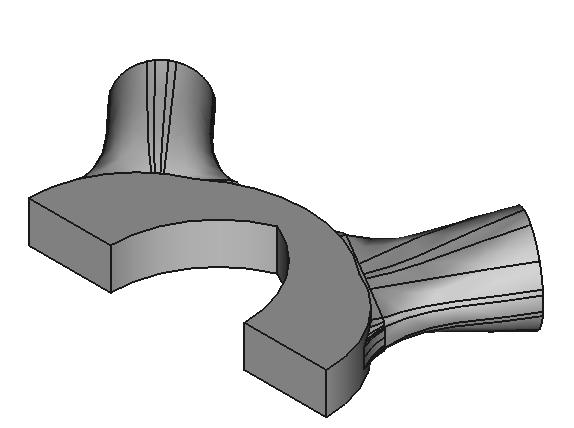
\includegraphics[width=\textwidth]{motor_cad1.png}
    \end{subfigure}
    \begin{subfigure}{0.4\textwidth}
        \centering
        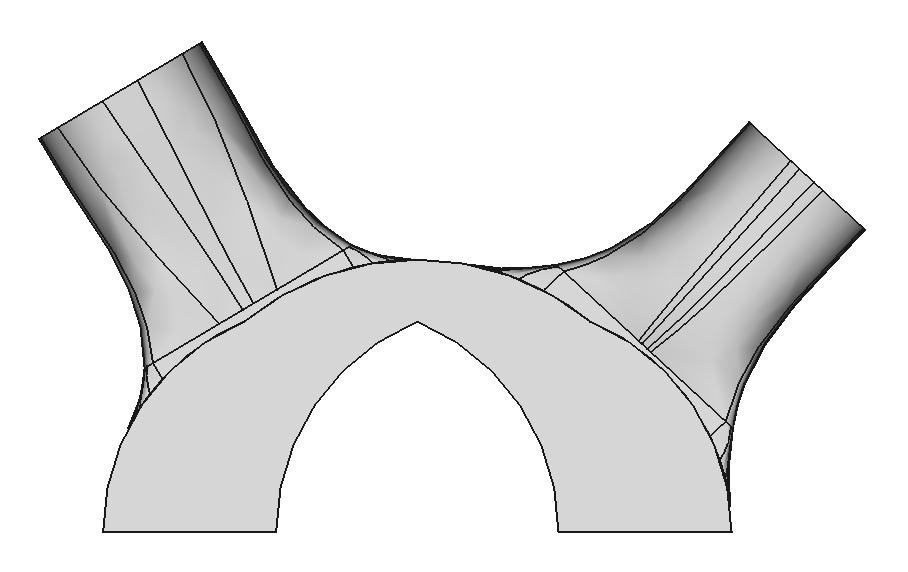
\includegraphics[width=\textwidth]{motor_cad2.png}
    \end{subfigure}
  \caption{CAD Primer Iteración}\label{fig:motor_cad1}
\end{figure}

En la figura~\ref{fig:motor_cad2} (a) y (b) se muestran las superficies
correspondientes a los puertos de admisión y escape respectivamente, la ranura
del lado del motor es de altura constante e igual a $h_{puerto} = \frac{2}{3}
h_{camara} = \lua{tex.print(myData.hp)}$ mm hasta alcanzar los extremos de la
misma en donde se reduce parcialmente.

\begin{figure}
  \centering
    \begin{subfigure}{0.8\textwidth}
        \centering
        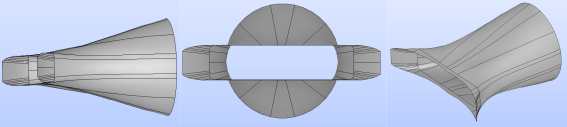
\includegraphics[width=\textwidth]{vistas_admision.png}
        \caption{Puerto de Admsisión.}
    \end{subfigure}
    \begin{subfigure}{0.8\textwidth}
        \centering
        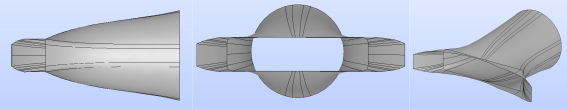
\includegraphics[width=\textwidth]{vistas_escape.png}
        \caption{Puerto de Escape.}
    \end{subfigure}
  \caption{CAD Primer iteración (vistas fuera de escala).}\label{fig:motor_cad2}
\end{figure}
